\setcounter{chaptercntr}{3}

\sectionbreak \section*{
  \gostTitleFont
  \redline
  \thechaptercntr .
  АНАЛИЗ И ОБРАБОТКА ДАННЫХ МОЕЧНОЙ СТАНЦИИ
}

\titlespace

\subsection*{ 
  \gostTitleFont
  \redline
  \thechaptercntr .\thesubchaptercntr \spc
  Анализ и визуализация исходных данных технологического процесса
} \addtocounter{subchaptercntr}{1}

\subtitlespace

{\gostFont
	
	\par \redline Одним из ключевых понятий данной работы является понятие временных рядов. Временные ряды {--} это некоторая последовательность, каждый элемент из которой состоит из двух или более параметров, один из которых обязательно должен обозначать время. Причём, все эти элементы в последовательности расположены в хронологическом порядке, т.е. в порядке возрастания параметра времени. 
	
	\par \redline Параметр времени может быть представлен в разных форматах. Выбор формата времени зависит от задачи, удобства использования, длительности, в пределах которой будут собираться данные, а также от требуемой точности. Например, в случае если данные фиксируются раз в день, то хорошо подойдёт отсчёт времени по дням с указанием месяца и года. Если же данные фиксируются в определённые моменты дня, то к вышеописанному стоит прибавить указание часа и минуты фиксации. При необходимости можно указывать и секунды, и миллисекунды. Но что, если нам не особо-то и важно знать, в какой год, месяц или день это происходило, когда нам важно знать, сколько прошло времени от начала того или иного процесса? Тогда, нам скорее подойдёт формат дискретного времени. С помощью этого формата можно узнать длительность процесса в единственной выбранной нами единице измерения времени. Например, если мы сохраняем время в секундах, то 1000-ча секунд сохранит свой формат 1000-чи секунд, время не будет переведено в 16-ать минут и 40-ок секунд. Всё это нам позволяет не привязываться к датам, которые не особо-то и влияют на технологический процесс промышленного оборудования.
	
	\par \redline Остальные параметры могут уже характеризовать или описывать какой-либо процесс или процессы, причём даже не обязательно одного элемента, а даже целой системы элементов. Так, например, когда наш элемент последовательности состоит из двух признаков, а один из которых, как мы уже знаем, время, то второй, конечно же, уже будет обозначать характеристику или состояние изучаемого нами элемента. Но как только у нас появляется три или более признаков, тогда мы уже можем говорить о фиксации характеристик или состояний разных элементов изучаемой системы в один и тот же момент времени или же о фиксации характеристики или состояния одного из множества элементов системы, но с указание этого элемента, например, с помощью идентификационного номера элемента. Как можно убедиться, временные ряды дают весьма гибкую возможность описания процессов или систем относительно времени. 
	
	\par \redline Технологический процесс моечной станции как раз и представляет собой временной ряд, в котором имеется информация о показаниях различных датчиков в определённые моменты времени. Поэтому, говоря о данных технологического процесса пастеризационной установки, мы будем понимать, что они имеют форму временных рядов.
	
	\par \redline Работа с временными рядами технологического процесса делится на две части. Первая часть {--} это понимание структуры временного ряда, его закономерностей, таких как цикличность, тренд, сезонность и так далее, обработка данных временного ряда, визуализация данных, в общем, это всесторонний анализ временного ряда. Если опускать различные математические, статистические и подобные подробности, то анализ также может дать нам возможность понять, как начинался процесс, как шёл и развивался и на чём он закончился или остановился на данном моменте времени.  Строго говоря, нейронным сетям, как и исследователям временных рядов, тоже необходимо это понять, чтобы выполнить вторую часть работы, а именно, составление прогноза, что, зачастую, и является основной задачей работы с временным рядом. Да, анализ данных временного ряда технологического процесса делается с целью понять, что будет происходить с этим процессом дальше.

  \par \redline Данные, которые мы будет использовать для обучения, имеют форму временных рядов, состоящих из трёх параметров. Первый параметр {--} это идентификатор датчика или исполняющего устройства, который в дальнейшем мы будем называть просто сид. Второй параметр {--} это дискретный момент времени, измеряемый в секундах. Третий параметр {--} значение датчика. 

  \par \redline Имеющиеся данные, описывающие технологический процесс моечной станции, содержит информацию от восьми различных датчиков. Информация по датчикам обозначена в таблице \thechaptercntr .\thetablecntr. 
  
  \par \redline Для начала определим, достаточно ли данных для обучения. Имеется 7 файлов формата .csv, которые хранят информацию о технологическом процессе моечной станции в течении 66734344 секунд или около 773 дней. За такой промежуток времени имеется около 2 миллионов данных различных сидов. Поэтому можно заявлять, что данных для проекта машинного обучения более чем достаточно, а потому имеется возможность обеспечить достаточную обобщающую способность модели.
  
  \par \redline Данные описывают состояние моечной станции круглые сутки в течении почти двух с половиной лет. Это нам позволяет говорить о большом покрытии данных. Это значит, что данные отражают все состояния объекта. Также мы можем говорить об информативности данных, поскольку она отражает реальный технологический процесс.
  
  \par \redline Для прояснения дальнейших моментов, необходимо обратить внимание на то, что данные были собраны с помощью датчиков, поэтому данные являются надёжными и не подверженными к большинству видов смещений – несогласованность данных с явлением, которые эти данные описывают.  Однако, эти данные всё-таки могут быть подвержены систематическому смещению, возникающее при измерениях или наблюдениях с помощью некоторого устройства, поскольку качество и характеристики устройства влияют на качество самих данных. Однако, мы можем игнорировать данное смещение, поскольку дальнейшая работа будет построена с теми же датчиками, а потому мы может говорить и о ещё одной черте качественных данных, а именно о том, что данные отражают реальный входы. Это значит, что будущая сеть будет обучаться на данных, представленных в таком виде, в котором они будут в последствии приходить на входы сети. В будущем будет упомянуто данное свойство и будет сказано о некоторых подводных камнях, связанных с этим.
  
  \par \redline Необходимо отметить, что данные не являются результатом обратной связи, т.е. не являются результатом самой модели, поскольку при сборе данных модели ещё не существовало.
  
  \par \redline
  
  \rotatebox{90}{ %это обеспечивает поворот любого объекта
  	\begin{minipage}{1.5\linewidth}
  		\begin{center}
  			\par \redline \phantom{hellow} 
  			\par \redline \phantom{hellow} 
  			\par \redline \phantom{hellow} 
  			\par \redline \phantom{hellow} 
  			\par \redline \phantom{hellow} 
  			\par \redline \phantom{hellow} 
  			\par \redline \phantom{hellow}
  			\par \redline \phantom{hellow}
  			\par \redline \phantom{hellow}
  			\par \redline \phantom{hellow} 
  			\begin{flushleft}
  			\par \centering Таблица \thechaptercntr .\thetablecntr \spc {--} Описание информации получаемой с датчиков с разбиением по номерам получаемой информации
  		\end{flushleft} \addtocounter{thetablecntr}{1}  
  			\centering
  			\begin{tabular}{|c|p{7cm}|c|}
  				\hline
  				cid & \centering Описание &  Размерность \\
  				\hline
  				1 & \centering Температура на подаче & \si{\celsius}  \\
  				\hline
  				2 & \centering Задание температура на подаче & \si{\celsius} \\
  				\hline
  				3 & \centering Температуры на возврате & \si{\celsius} \\
  				\hline
  				&  Задание температура на возврате  (температура на подаче - 10) &  \si{\celsius} \\
  				\hline
  				4 & \centering Поток &  0/1 (есть/нет) \\
  				\hline
  				5 & \centering Подогревающий клапан (открытие) & 0-100 (0 - полностью закрыт, 100 - полностью открыт) \\
  				\hline
  				6 & \centering Расход на подаче & \si{м\tothe{3}/час} \\
  				\hline
  				7 & \centering Задание расхода на подаче & \si{м\tothe{3}/час} \\
  				\hline
  				8 & \centering Подающий насос (мощности) &  0-100 (0 - минимальная мощность, 100 - максимальная мощность) \\
  				\hline
  			\end{tabular}
  		\end{center}
  \end{minipage}} 

  \par 
}

\subtitlespace

\subsection*{ 
  \gostTitleFont
  \redline
  \thechaptercntr .\thesubchaptercntr \spc
  Обработка данных и их подготовка к прогнозированию
} \addtocounter{subchaptercntr}{1}

\subtitlespace

{\gostFont

  \par \redline При обработке данных необходимо учитывать особенности данных применяемых при прогнозировании. Любые данные нуждаются в обработке перед любым применением.  Цели такой обработки могут быть разные, например: 
  
  \begin{itemize}[leftmargin=2.15cm, labelwidth=0.65cm, labelsep=0.0cm] 
  	
  	\item[\theitemcntr. ] Приведение данных к табличному виду.
  	\addtocounter{itemcntr}{1}
  	
  	\item[\theitemcntr. ] Аппроксимация данных.
  	\addtocounter{itemcntr}{1}
  	
  	\item[\theitemcntr. ] Уменьшение размерности данных.
  	\addtocounter{itemcntr}{1}
  	
  	\item[\theitemcntr. ] Разделение данных.
  	\addtocounter{itemcntr}{1}
  	
  	\item[\theitemcntr. ] Устранение аномалий данных.
  	\addtocounter{itemcntr}{1}
  	
  	\item[\theitemcntr. ] Устранение некорректных данных.
  	\addtocounter{itemcntr}{1}
  	
  	\setcounter{itemcntr}{1}
  \end{itemize}

  \par \redline Поговорим о хранении данных. Начальные данные хранятся в файлах формата .csv. Данный формат файлов является распространенным для хранения данных, представленных в форме временных рядов. В них данные хранятся в следующем виде: 
  
  \begin{Center}
  <сид>;<время>;<значение>. 
  \end{Center}

  \par \redline В дальнейшем данный вид данных мы будем обозначать как ocdf-формат данных. Преимуществом хранения данных в таких файлах является их доступность для любых программ или языков. Однако такие файлы занимают большой объём, а также при работе с такими файлами чтение или запись информации занимает большое количество времени.  

  \par \redline Для решения основных проблем при работе с файлами формата .csv, было принято решение использовать бинарные файлы формата .bin для хранения данных. Это дало возможность уменьшить занимаемый объём файлов, но самое главное, это позволило значительно сократить время для записи или чтения информации, связанное с тем, что нет необходимости конвертировать данные из бинарного в текстовый формат и наоборот.

  \par \redline В ходе работы с моделью возможно не будет необходимости работать со всеми сидами, а только с определёнными. Для того, чтобы не задействовать оперативную память зря, необходимо разделить данные по сидам.   

  \par \redline Для формирования различных наборов данных необходима возможность обрезать данные до необходимого нам диапазона или количества. Для более полного понимая смысла обрезки данных в очередной раз обратимся к инженерии машинного обучения: весь набор данных делится на обучающий, контрольный и тестовый наборы. Обучающий набор используется для непосредственного обучения модели. На контрольном наборе проверяется качество модели и подбираются её параметры, другими словами, настраивается модель. На тестовом наборе проверяется работа сети и делается вердикт о готовности модели. 

  \par \redline Для формирования различных наборов данных как раз и нужны различные способы обрезки данных, позволяющие отбросить данные как справа, так и слева. 
 
  \par \redline Также необходима возможность добавлять новые данные, чтобы при обучении сеть, которая учитывает зависимости между различными датчиками, была обеспечена данными необходимых сидов.  

  \par \redline Учитывая особенности вида данных, которые поступают на предиктовый детектор системы Kaspersky MLAD, а также ввиду того, что данная модель будет работать в режиме реального времени и данные будут поступать через некоторый промежуток времени, то необходимо сделать так, чтобы начальные данные также были равноудалены друг от друга относительно оси времени. Однако, взаимное удаление точек по оси времени в начальных данные не постоянно. Эти диапазоны необходимо выровнять, чтобы повысить схожесть реальных входов и входов при обучении модели. Другими словами, необходимо преобразовать начальный данные в такие данные, в которых каждое значение времени представляло собой арифметическую прогрессию:

  
  	\formulaspace \par \redline 
  $ t_i = t_0 + i \times r $
  \hfill (\thechaptercntr .\theformulacntr) \redline
  \formulaspace \addtocounter{formulacntr}{1}

  \begin{tabular}{p{0,875cm}p{0,3cm}p{15,175cm}}
  	& где  & $\textrm{t}_\textrm{0}$ {--} начальное значение времени; \\
  	&      & $\textrm{r}}$ {--} необходимое расстояние между точками, представляющее собой некоторую константу, которую может задать пользователь; \\
  	&      & $\textrm{i}$ {--} номер точки, итерации, элемента прогрессии;  \\
  	&      & $\textrm{t}_\textrm{i}$ {--} i-ыт элемент прогрессии.  \\
  \end{tabular} 

  \par \redline Теперь осталось определить значение ординаты для каждого рассчитанного значения времени. Для этого было принято решение воспользоваться аналитической геометрией и взять за основу уравнение прямой, проходящей через две точки.  
  
  	\formulaspace \par \redline 
  $ \frac{x - x_1}{x_2 - x_1} = \frac{y - y_1}{y_2 - y_1} $
  \hfill (\thechaptercntr .\theformulacntr) \redline
  \formulaspace \addtocounter{formulacntr}{1}

  \par \redline где точка $\left(х, у\right)$ – это точка, которую необходимо найти между точками $\left(х_1, у_1\right)$ и $\left(х_2, у_2\right)$, взятых из реальных данных. При этом, известно, что $х_1 \leq x \leq x_2$. 

  \par \redline Для определение ординаты для i-того элемента прогресии необходимо взять две ближайших точки из реальных данных относительно оси абсцисс к искомой точке. Тогда получим выражение для определение ординаты:
  
  	\formulaspace \par \redline 
  $ y = \left(\frac{\left(x - x_1\right) \times \left(y_2 - y_1\right)}{x_2 - x_1}\right) + y_1 $
  \hfill (\thechaptercntr .\theformulacntr) \redline
  \formulaspace \addtocounter{formulacntr}{1}

  \par \redline Таким образом можно получить аппроксимированные данные, где взаимное удаление между двумя соседними точками будет везде постоянным.  

  \par \redline Благодаря возможности выравнивания диапазонов по оси абсцисс, появляется возможность создать, так называемые, аккуратные данные – данные представленные в виде упорядоченной таблицы без каких-либо «дыр». Однако, если попытаться перевести имеющиеся данные в табличный формат, который в последствии мы будем называть tdf форматом, то мы обнаружим, что начальные данные содержат информацию о значениях датчика при неповторяющихся уникальных значениях времени. Это значит, что если для некоторого датчика определено его значение в некоторый момент времени в начальных данных, то значение другие датчиков в этот же момент времени не известно. Для решения данной проблемы нам помогут операции парсинга и выравнивания диапазонов по оси абсцисс. Чтобы преобразовать данные формата ocdf в данные формата tdf необходимо выполнить несколько последовательных действий. 

  \par \redline Для начала необходимо убедиться, что данные формата ocdf содержат в себе данные всех сидов, а после распарсить данные по сидам. Затем обрезать все последовательности распарсенных данных с их начала и до максимального значения времени первых элементов последовательности распарсенных данных, также с минимального значения времени последних элементов последователи распарсенных данных до конца всех последовательностей распарсенных данных. Если в обрезаемой последовательности нет точки с граничным значением времени, тогда необходимо найти эту точку средствами уравнения прямой через две точки, описанной выше. Далее выровнять диапазоны по оси абсцисс для всех расперсенных данных. В заключении требуется соединить полученные данные в одну последовательность следующего вида. Формат tdf выглядит следующим образом:

  \begin{Center}
  <время>;<ЗД1>;< ЗД2>;< ЗД3>;< ЗД4>;< ЗД5>;< ЗД6>
  \end{Center}

  \par \redline где, ЗДН – значение датчика под номером Н. 

  \par \redline Выполнив алгоритм, мы получаем аккуратные данные в табличном виде. Хранить их предпочтительно в бинарном виде, поскольку в формате .csv такие данные будут занимать очень много места, да и время на их чтение или запись будет довольно-таки немаленьким. 

  \par \redline Учитывая некоторые особенности активирующих функций, некоторые модели будут содержать в себе встроенные модули преобразования данных из одного диапазона по оси ординат в эквивалентные данные из другого диапазона по оси ординат и наоборот, сохраняя значения по оси абсцисс. Такую операцию мы будет в дальнейшем называть скейлингом.

  \par \redline Данная задача выглядит следующим образом: пусть есть $y \in \left[a; b\right]$, а необходимо преобразовать $y$ в эквивалентное значение $z \in \left[c; d\right]$. Тогда для операции скейлинга имеем следующее выражение:

  	\formulaspace \par \redline 
  $ z = \frac{\left(y - a\right) \times \left(b - a\right)}{d - c} + c $
  \hfill (\thechaptercntr .\theformulacntr) \redline
  \formulaspace \addtocounter{formulacntr}{1}
  

  \par \redline А для того, чтобы восстановить эти значения, т.е. провести операцию обратного скейлинга, необходимо использовать следующее выражение: 

	\formulaspace \par \redline 
$ y = \frac{\left(z - c\right) \times \left(d - c\right)}{b - a} + a $
\hfill (\thechaptercntr .\theformulacntr) \redline
\formulaspace \addtocounter{formulacntr}{1}

  \par \redline Операции скейлинга предполагают те модели, выходные элементы которых используют активирующие функции, имеющие горизонтальные асимптоты. Другими словами, активирующие функции, ограниченные по оси ординат. В таком случае, перед обучение или прогнозированием данных, будет проведена операция скейлинга, после основная операция, а в завершении операция обратного скейлинга. Т.к. данные уже изучены, можно с полной уверенность сказать, что операцию скейлинга для данных по оси ординат мы можем провести.
  
  \par \redline В итоге обработки данных получаем данные, выровненные по времени и приведенные к табличной форме. Визуализацию данных представлена на рисунках \thechaptercntr.\theimagecntr {--} \thechaptercntr.8.

  \par
  
    \begin{sidewaysfigure}
  	\centering
  	\def\svgwidth{\textwidth}
  	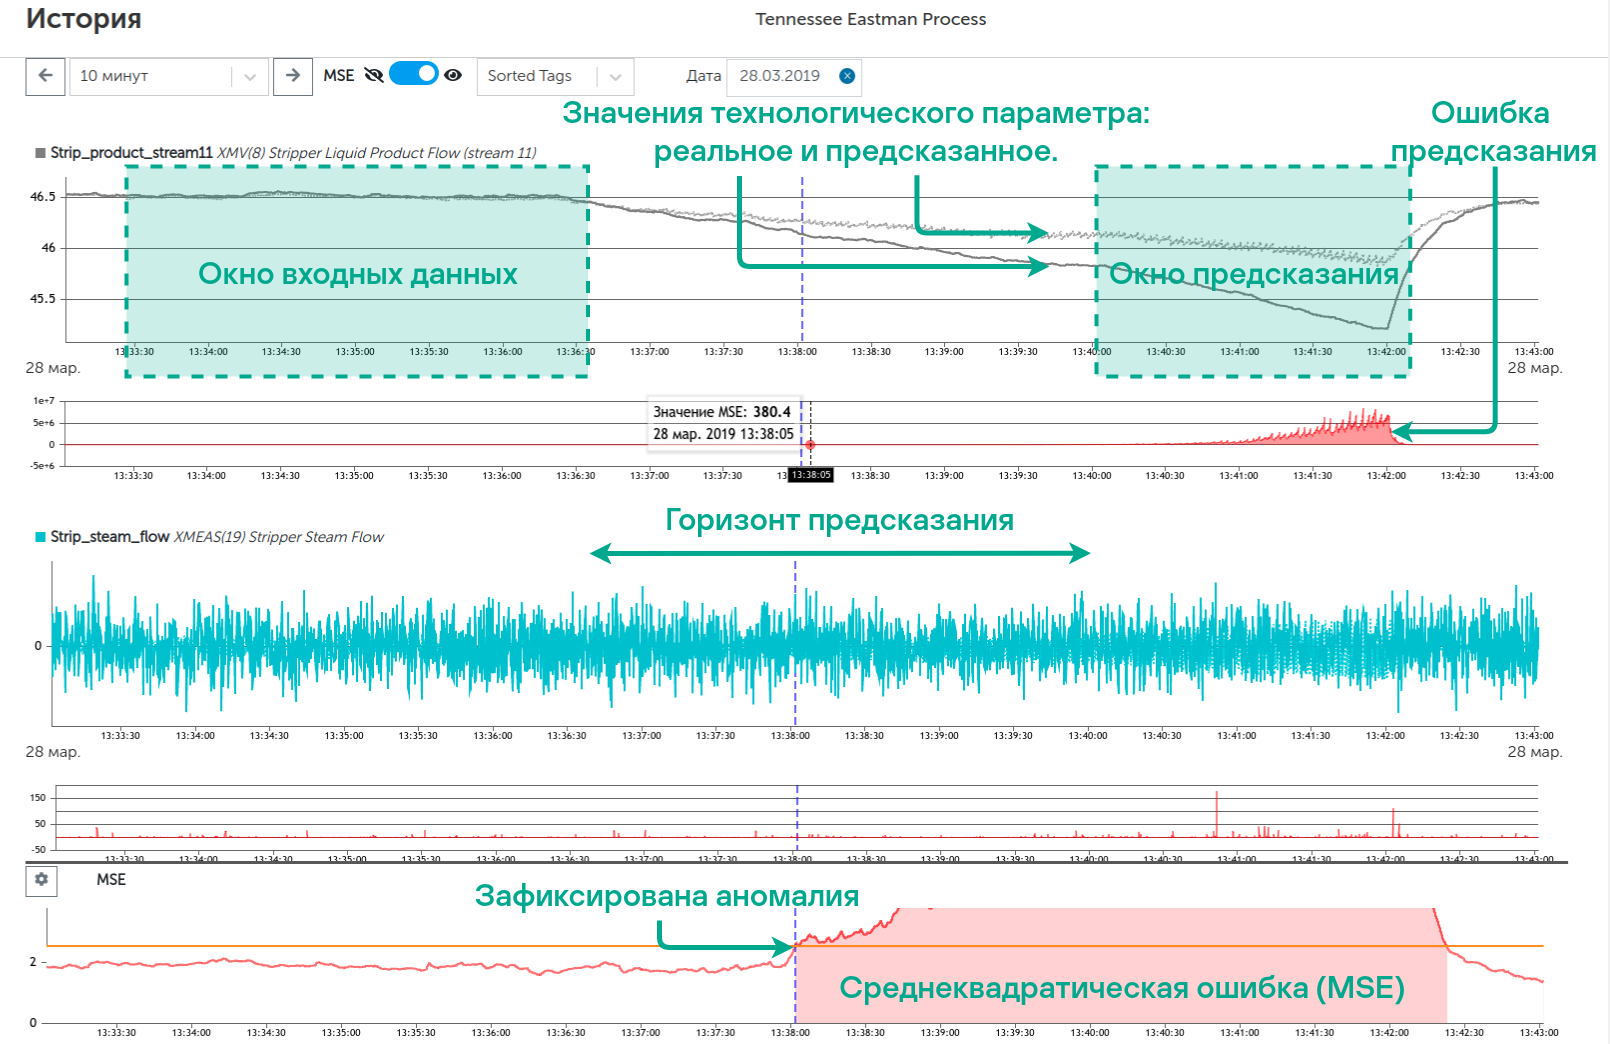
\includegraphics[scale=0.6]{images/MLADex.png}
  	\caption*{\gostFont Рисунок \thechaptercntr .\theimagecntr \spc {--} Пример работы предиктового детектора системы Kaspersky MLAD}
  	\label{fig:MLADBlackBox}
  \end{sidewaysfigure} \addtocounter{imagecntr}{1}
  
     \begin{sidewaysfigure}
  	\centering
  	\def\svgwidth{\textwidth}
  	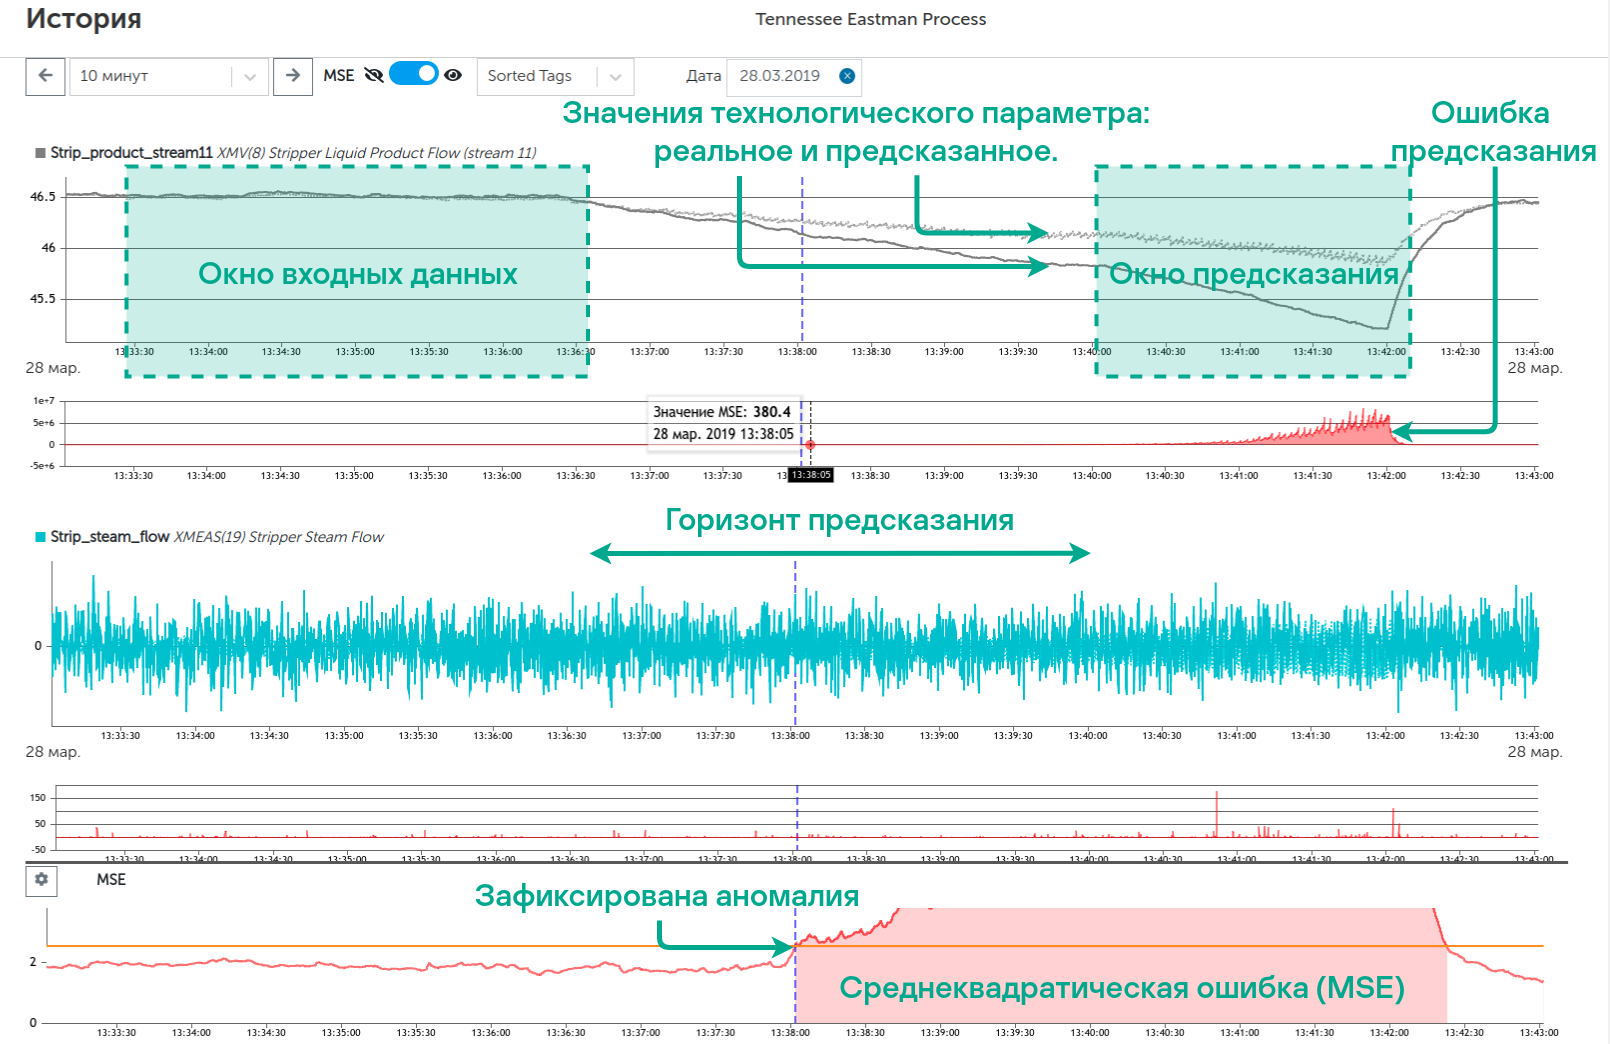
\includegraphics[scale=0.6]{images/MLADex.png}
  	\caption*{\gostFont Рисунок \thechaptercntr .\theimagecntr \spc {--} Пример работы предиктового детектора системы Kaspersky MLAD}
  	\label{fig:MLADBlackBox}
  \end{sidewaysfigure} \addtocounter{imagecntr}{1}
  
     \begin{sidewaysfigure}
  	\centering
  	\def\svgwidth{\textwidth}
  	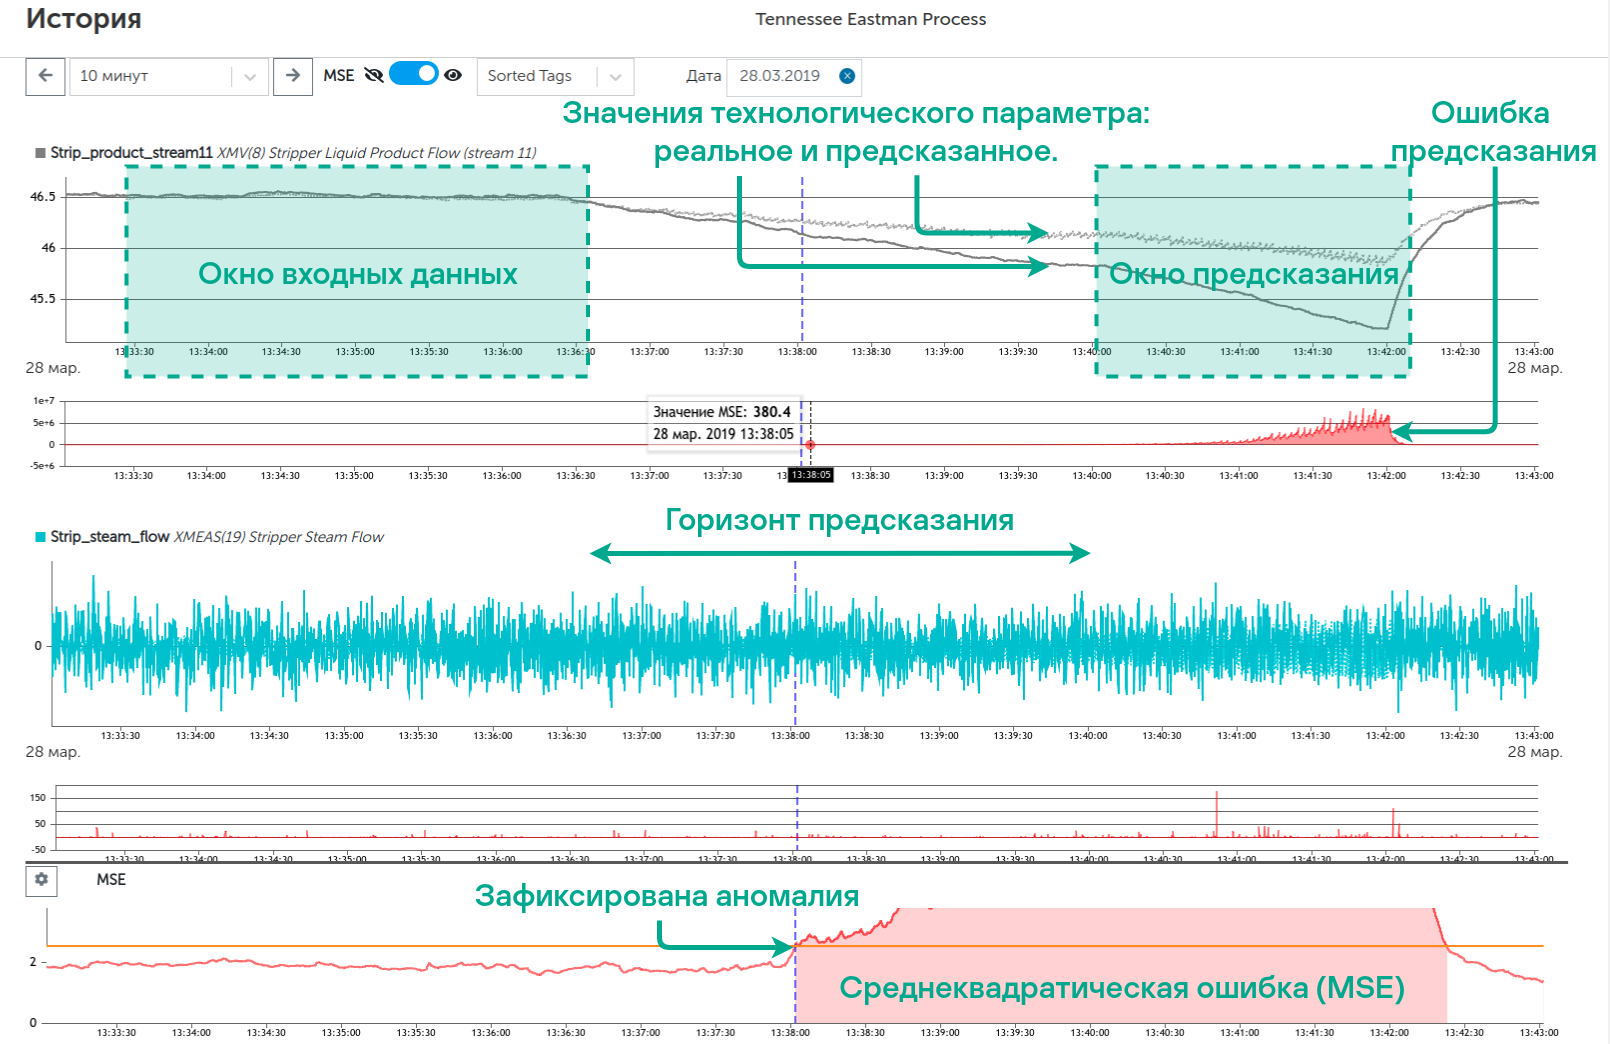
\includegraphics[scale=0.6]{images/MLADex.png}
  	\caption*{\gostFont Рисунок \thechaptercntr .\theimagecntr \spc {--} Пример работы предиктового детектора системы Kaspersky MLAD}
  	\label{fig:MLADBlackBox}
  \end{sidewaysfigure} \addtocounter{imagecntr}{1}
  
     \begin{sidewaysfigure}
  	\centering
  	\def\svgwidth{\textwidth}
  	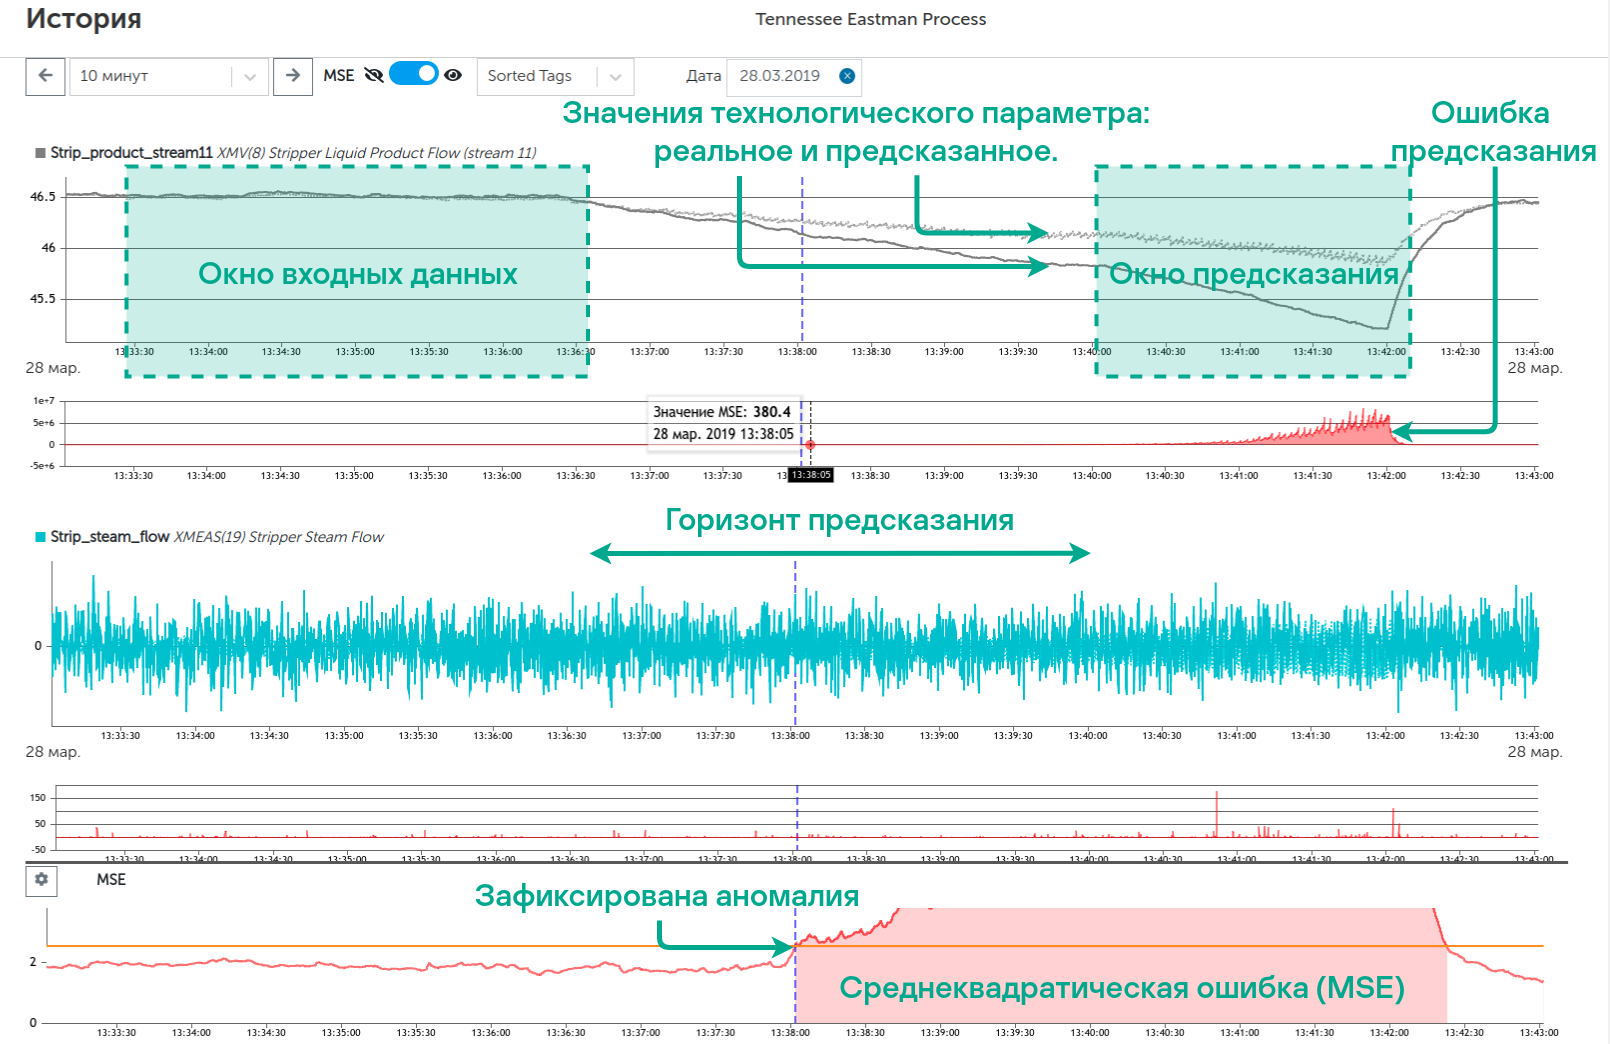
\includegraphics[scale=0.6]{images/MLADex.png}
  	\caption*{\gostFont Рисунок \thechaptercntr .\theimagecntr \spc {--} Пример работы предиктового детектора системы Kaspersky MLAD}
  	\label{fig:MLADBlackBox}
  \end{sidewaysfigure} \addtocounter{imagecntr}{1}
  
     \begin{sidewaysfigure}
  	\centering
  	\def\svgwidth{\textwidth}
  	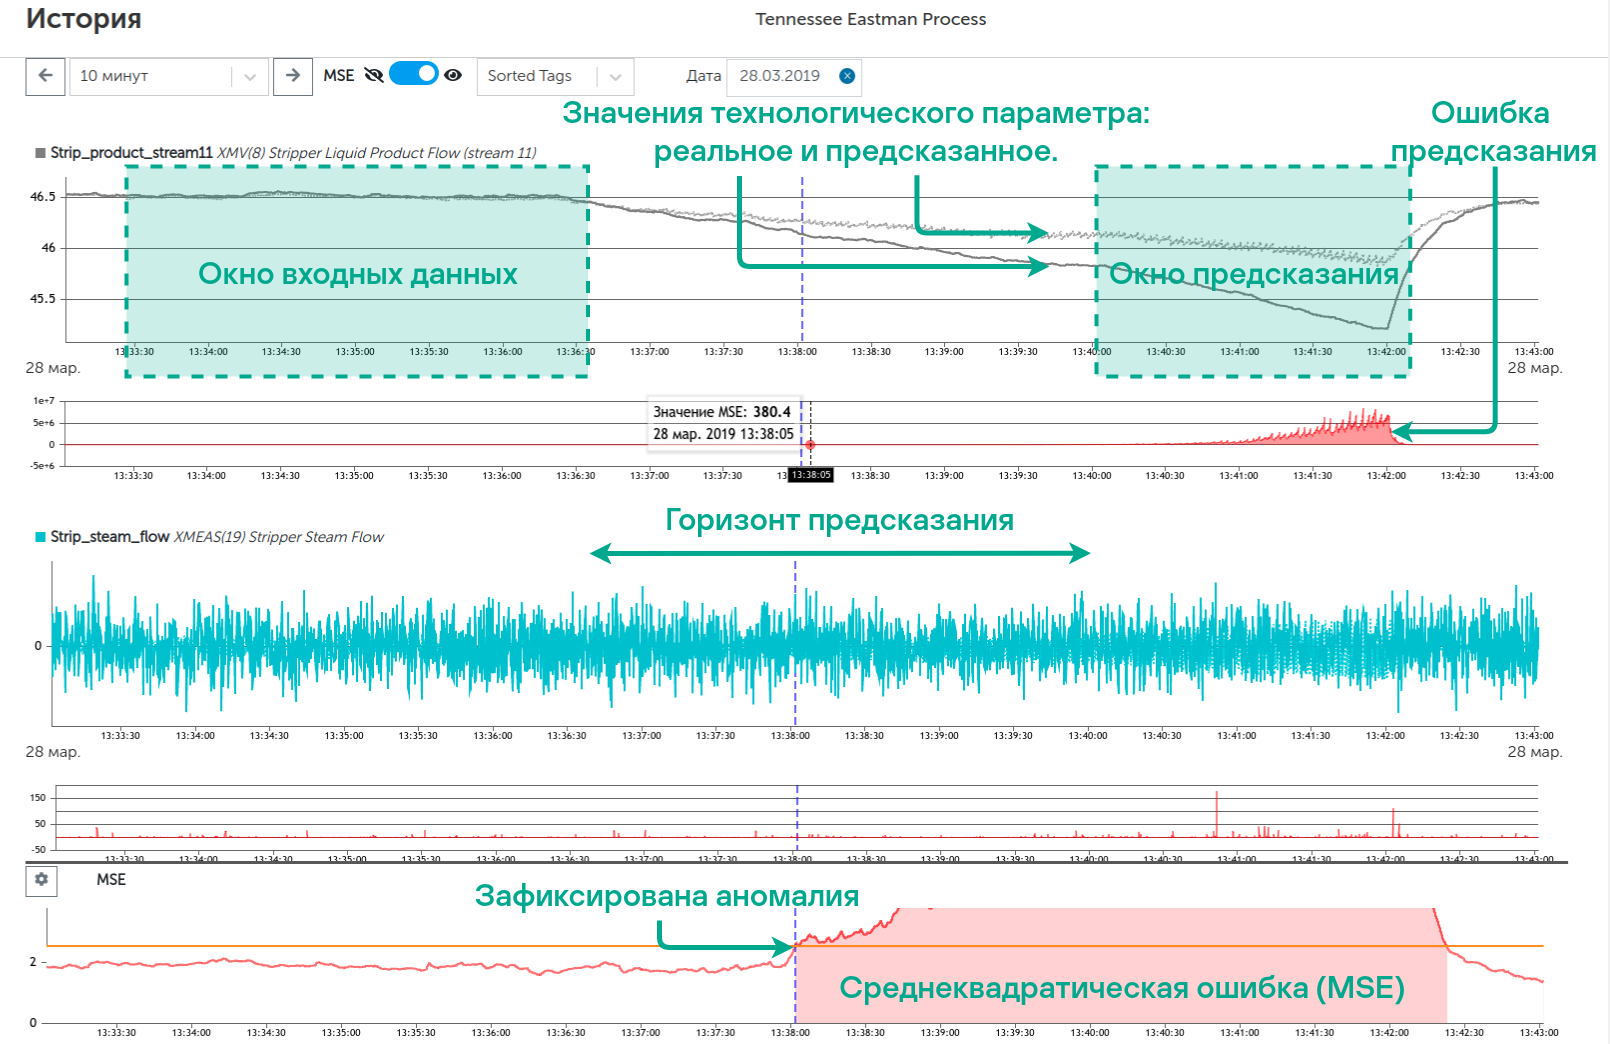
\includegraphics[scale=0.6]{images/MLADex.png}
  	\caption*{\gostFont Рисунок \thechaptercntr .\theimagecntr \spc {--} Пример работы предиктового детектора системы Kaspersky MLAD}
  	\label{fig:MLADBlackBox}
  \end{sidewaysfigure} \addtocounter{imagecntr}{1}
  
     \begin{sidewaysfigure}
  	\centering
  	\def\svgwidth{\textwidth}
  	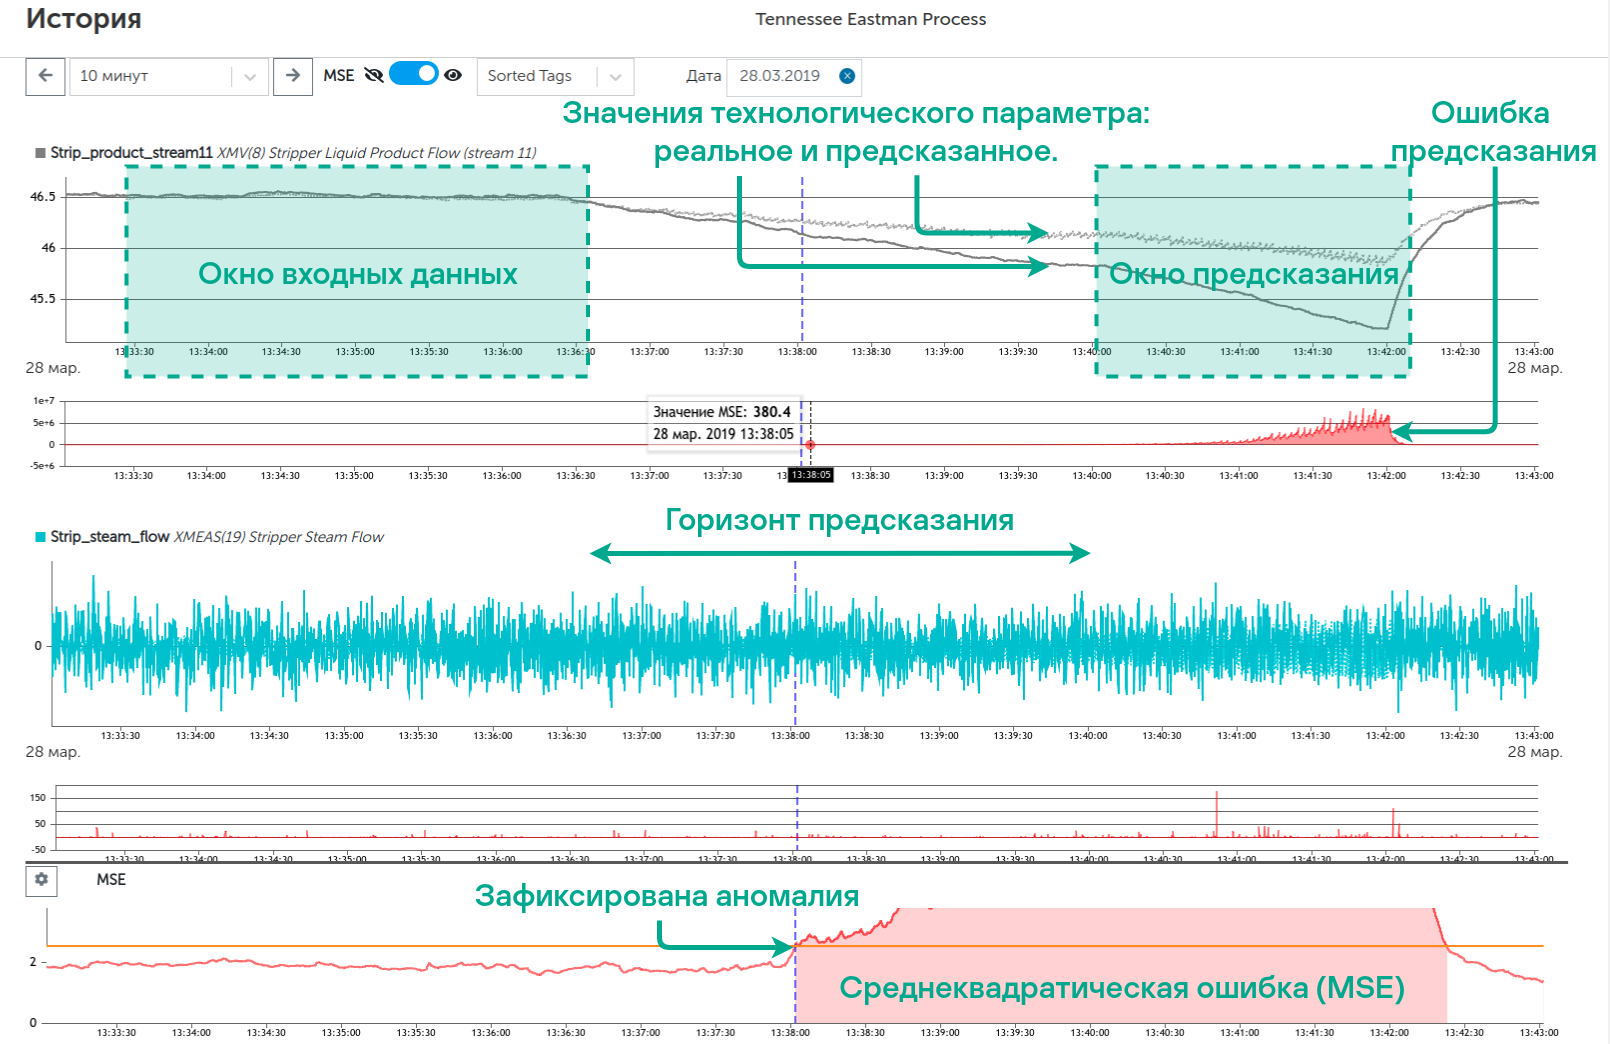
\includegraphics[scale=0.6]{images/MLADex.png}
  	\caption*{\gostFont Рисунок \thechaptercntr .\theimagecntr \spc {--} Пример работы предиктового детектора системы Kaspersky MLAD}
  	\label{fig:MLADBlackBox}
  \end{sidewaysfigure} \addtocounter{imagecntr}{1}
  
     \begin{sidewaysfigure}
  	\centering
  	\def\svgwidth{\textwidth}
  	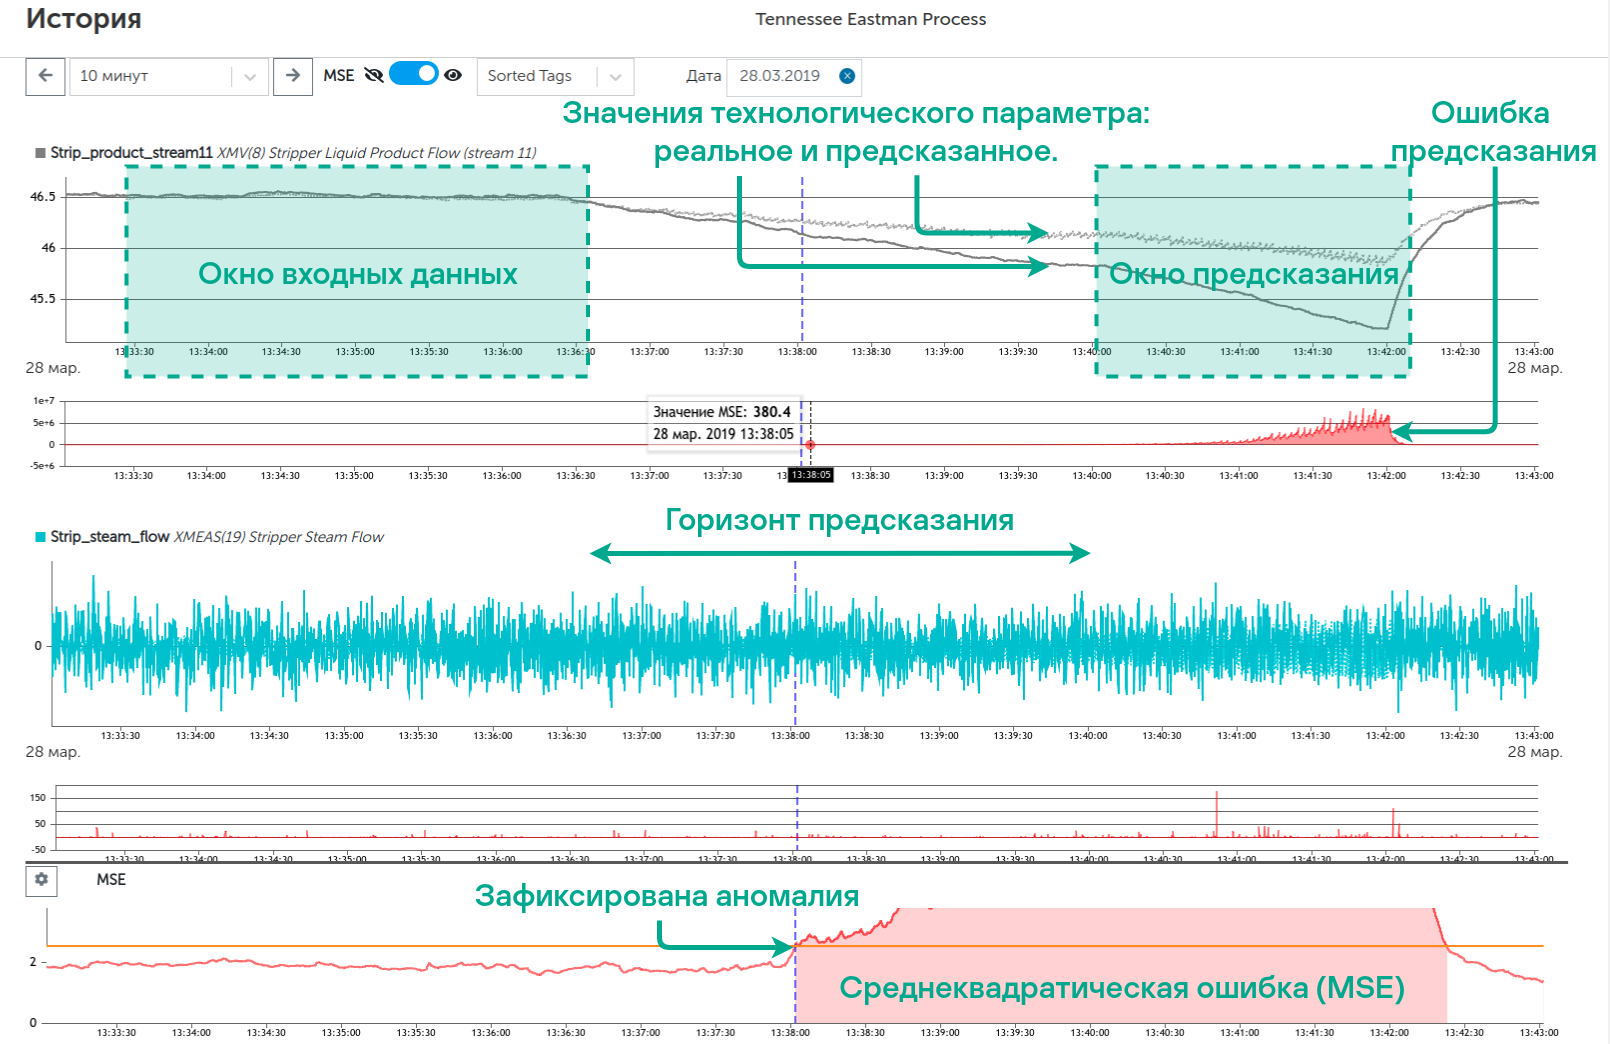
\includegraphics[scale=0.6]{images/MLADex.png}
  	\caption*{\gostFont Рисунок \thechaptercntr .\theimagecntr \spc {--} Пример работы предиктового детектора системы Kaspersky MLAD}
  	\label{fig:MLADBlackBox}
  \end{sidewaysfigure} \addtocounter{imagecntr}{1}
  
     \begin{sidewaysfigure}
  	\centering
  	\def\svgwidth{\textwidth}
  	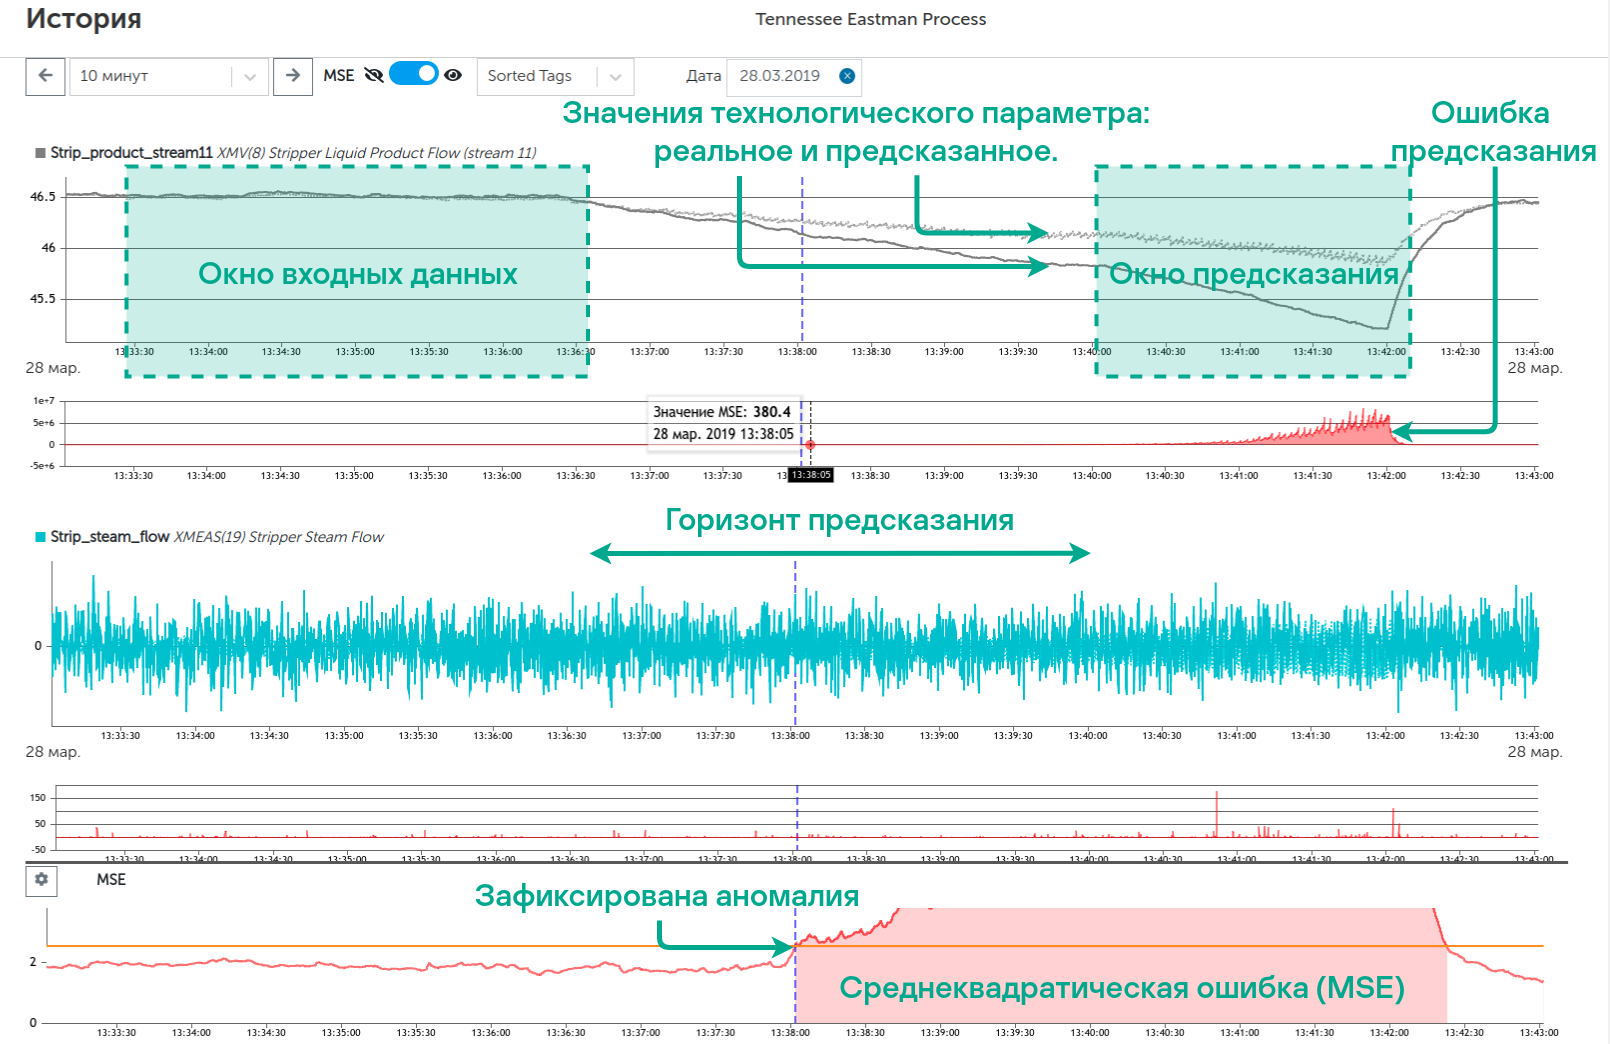
\includegraphics[scale=0.6]{images/MLADex.png}
  	\caption*{\gostFont Рисунок \thechaptercntr .\theimagecntr \spc {--} Пример работы предиктового детектора системы Kaspersky MLAD}
  	\label{fig:MLADBlackBox}
  \end{sidewaysfigure} \addtocounter{imagecntr}{1}
  
 
  
}

\setcounter{subchaptercntr}{1}
\setcounter{formulacntr}{1}
\setcounter{imagecntr}{1}
\setcounter{tablecntr}{1}
